\chapter{Introduction}
\label{ch:cta}

The Cherenkov Telescope Array will be the most sophisticated experiment in the field of ground-based gamma-ray astronomy to date.
The book \enquote{Science with the Cherenkov Telescope Array} published in 2019~\cite{cta:science} gives an exhaustive review 
of the scientific opportunities that arise with the CTA facility.
Once completed, CTA will be able to map the gamma-ray sky in an energy range from $\sim\SI{20}{GeV}$ to at least $\sim\SI{300}{TeV}$.
The unprecedented energy range will open a new window onto the very-high-energy sky. 
The lowest energies are invaluable to study distant extra-galactic sources of gamma rays. 
CTA's sensitivity in the \si{GeV} range avoids the absorption of distant sources by interaction with the extra-galactic background light.  
The largest energies will allow CTA to search for the extreme accelerators in our own galaxy which boost cosmic rays 
into the \si{PeV} energy range. 
CTA will be operated as a public observatory that serves the entire astronomy community. This is a new development for the astroparticle
community that opens up the possibilities for coordinated multi-wavelengths campaigns and exposure to the general public. Previously both observation schedules and 
observed data were only accessible to collaboration members. 

Observation of serendipitous transient events and response to multi-messenger alerts necessitates a wide field of view combined with 
a small angular resolution. The need for timely follow-up observations in the era of multi-messenger astronomy motivated the 
stringent requirements for the short timescale capabilities of CTA. The telescopes in the array are designed to reposition themselves 
to any point in the sky within 90 seconds at most. 
In response to the recent observation of gravitational waves with the LIGO and VIRGO detectors~\cite{gw2015},
the slewing times will be increased even further. 
The study of active galactic nuclei (AGN) will benefit immensely from the improved sensitivity in the lower energy range and the fast slewing times.
The observation of these distant highly variable objects can lead to a better understanding of black hole and jet dynamics. 
A full survey of the galactic plane and the Large Magellanic Clouds with CTA is planned. The quality of these surveys is limited by 
available observation time and angular resolution. CTA’s improved angular resolution compared to current instruments allows for better 
source separation in the densely populated Cygnus region in the center of the Milky Way. 
Other science goals probe the frontiers of current physics. CTA will search for Dark Matter, Axions, and quantum gravity effects.
To cover such a large span of observable energy ranges, CTA will host telescopes of three different sizes.
The Large Size Telescopes (LSTs) are, as the name suggests, the largest CTA telescopes.
The LSTs have a mirror diameter of 23m and a field of view of \SI{4.5}{\degree}. They are sensitive to the lowest part of the observed energy spectrum down to several \si{GeV}.
The first LST was built and officially inaugurated in October 2018. It is currently in its commissioning phase and its
mechanical structure and camera are being tested. Shower images have been successfully recorded by the LST camera.
The Medium Size Telescopes (MSTs) have a diameter of \SIrange{10}{12}{\metre} and a field of view (FoV) of \SIrange{6}{8}{\degree}.
Their highest sensitivity lies in the energy range of approximately \SI{100}{GeV} to \SI{1}{TeV}.
Two prototypes for the MST are under investigation at the moment. One is based in Adlershof near Berlin, where its mechanical 
structure is being overhauled. The MST-SCT dual-mirror prototype is located at the Fred Lawrence Whipple Observatory in Arizona and recently received 
funding to construct a first iteration of its \num{11000} pixel camera.
The Small Size Telescopes (SSTs) are built to observe the highest energies. 
They have large FoV of about \SI{10}{\degree} to image the brightest showers in the highest energy range above \SI{1}{TeV}.
Three SST prototypes have been built so far, two of which are already recording shower images. The SST-1M telescope in the city of Kraków in Poland, the ASTRI
telescope on the slopes of Mount Etna in Sicily, and the SST-GCT just outside of Paris.

The final CTA telescopes will be built at two observation sites, one in the northern hemisphere on the island of La Palma and one 
in Chile's Atacama dessert at the Paranal observatory. 
The array in the northern hemisphere will observe extra-galactic sources and some local pulsar wind nebulae. The southern array
will concentrate on galactic sources and features a larger field of view for a chance to catch 
rare galactic supernova explosions.  
Due to the nature of the ubiquitous power-law spectra, large collection areas are needed to catch the rare high-energy 
events above \SI{10}{TeV}. This is why CTA's southern array layout covers about \SI{4.5}{\square\kilo\metre} and consists of 50 to 70 
small SST type telescopes. The northern array is made up of 4 large LSTs and 10 to 15 medium-sized MST type telescopes.
\Cref{fig:cta_layout} shows the planned layouts of the northern and southern site. \Cref{fig:tel_renders} shows renderings 
of three CTA telescope prototypes. 

So far, the data for the Cherenkov Telescope Array only exists in simulated form.
The goal of the coming chapters will be to create a fully configurable and reproducible pipeline for CTA data analysis that 
matched the physics performance of previous CTA reference analyses.
This new analysis is based on the official CTA pipeline prototype \ctapipe, a \python-based program
which is developed in a public repository.
\Cref{ch:cta_analysis} lists all preprocessing steps that are needed to be performed on the raw, simulated, CTA data. 
In \cref{ch:ml}, the machine-learning methods for background suppression and energy estimation are explained.
The chapter also introduces the \aicttools software, which was developed to facilitate configurable machine learning
for IACTs.
A fully working prototype for a CTA real-time analysis is introduced in \cref{ch:rta}. It is capable of processing tens of thousands 
air shower events per second and can easily handle CTA's full data rate under real-time demands.
In \cref{ch:sensi} a full sensitivity curve for my CTA analysis is shown and compared to CTA’s reference curve.
Finally, \cref{ch:repro} contains a few remarks on the reproducibility of these results.

\begin{figure}
  \centering
  \includegraphics{build/array_layout.pdf}
  \caption[CTA layout at the northern and southern site]{ Planned array layout of the Paranal and La Palma sites. This is the layout used for the simulations throughout this document. 
  The CTA internal designation for this layout is HB9.
  The southern array consists of a total of \input{build/num_tel_south.txt}telescopes of which \input{build/num_sst_south.txt}are SST, \input{build/num_mst_south.txt}are MST, and
  \input{build/num_lst_south.txt}are LST type telescopes. The northern array on La Palma is made up of \input{build/num_mst_north.txt}MSTs  and 
  \input{build/num_lst_north.txt}LSTs. The array layout for the northern site is more irregular as it is located on a mountain top and has to adapt to the geological features of the 
  surface.   
  The Paranal site in Chile, on the other hand, is relatively flat. The layouts were optimized using large-scale simulations described in a paper by Tarek Hassan and others~\cite{cta_layout}.
  }
  \label{fig:cta_layout}
\end{figure}

\begin{figure}
  \centering
  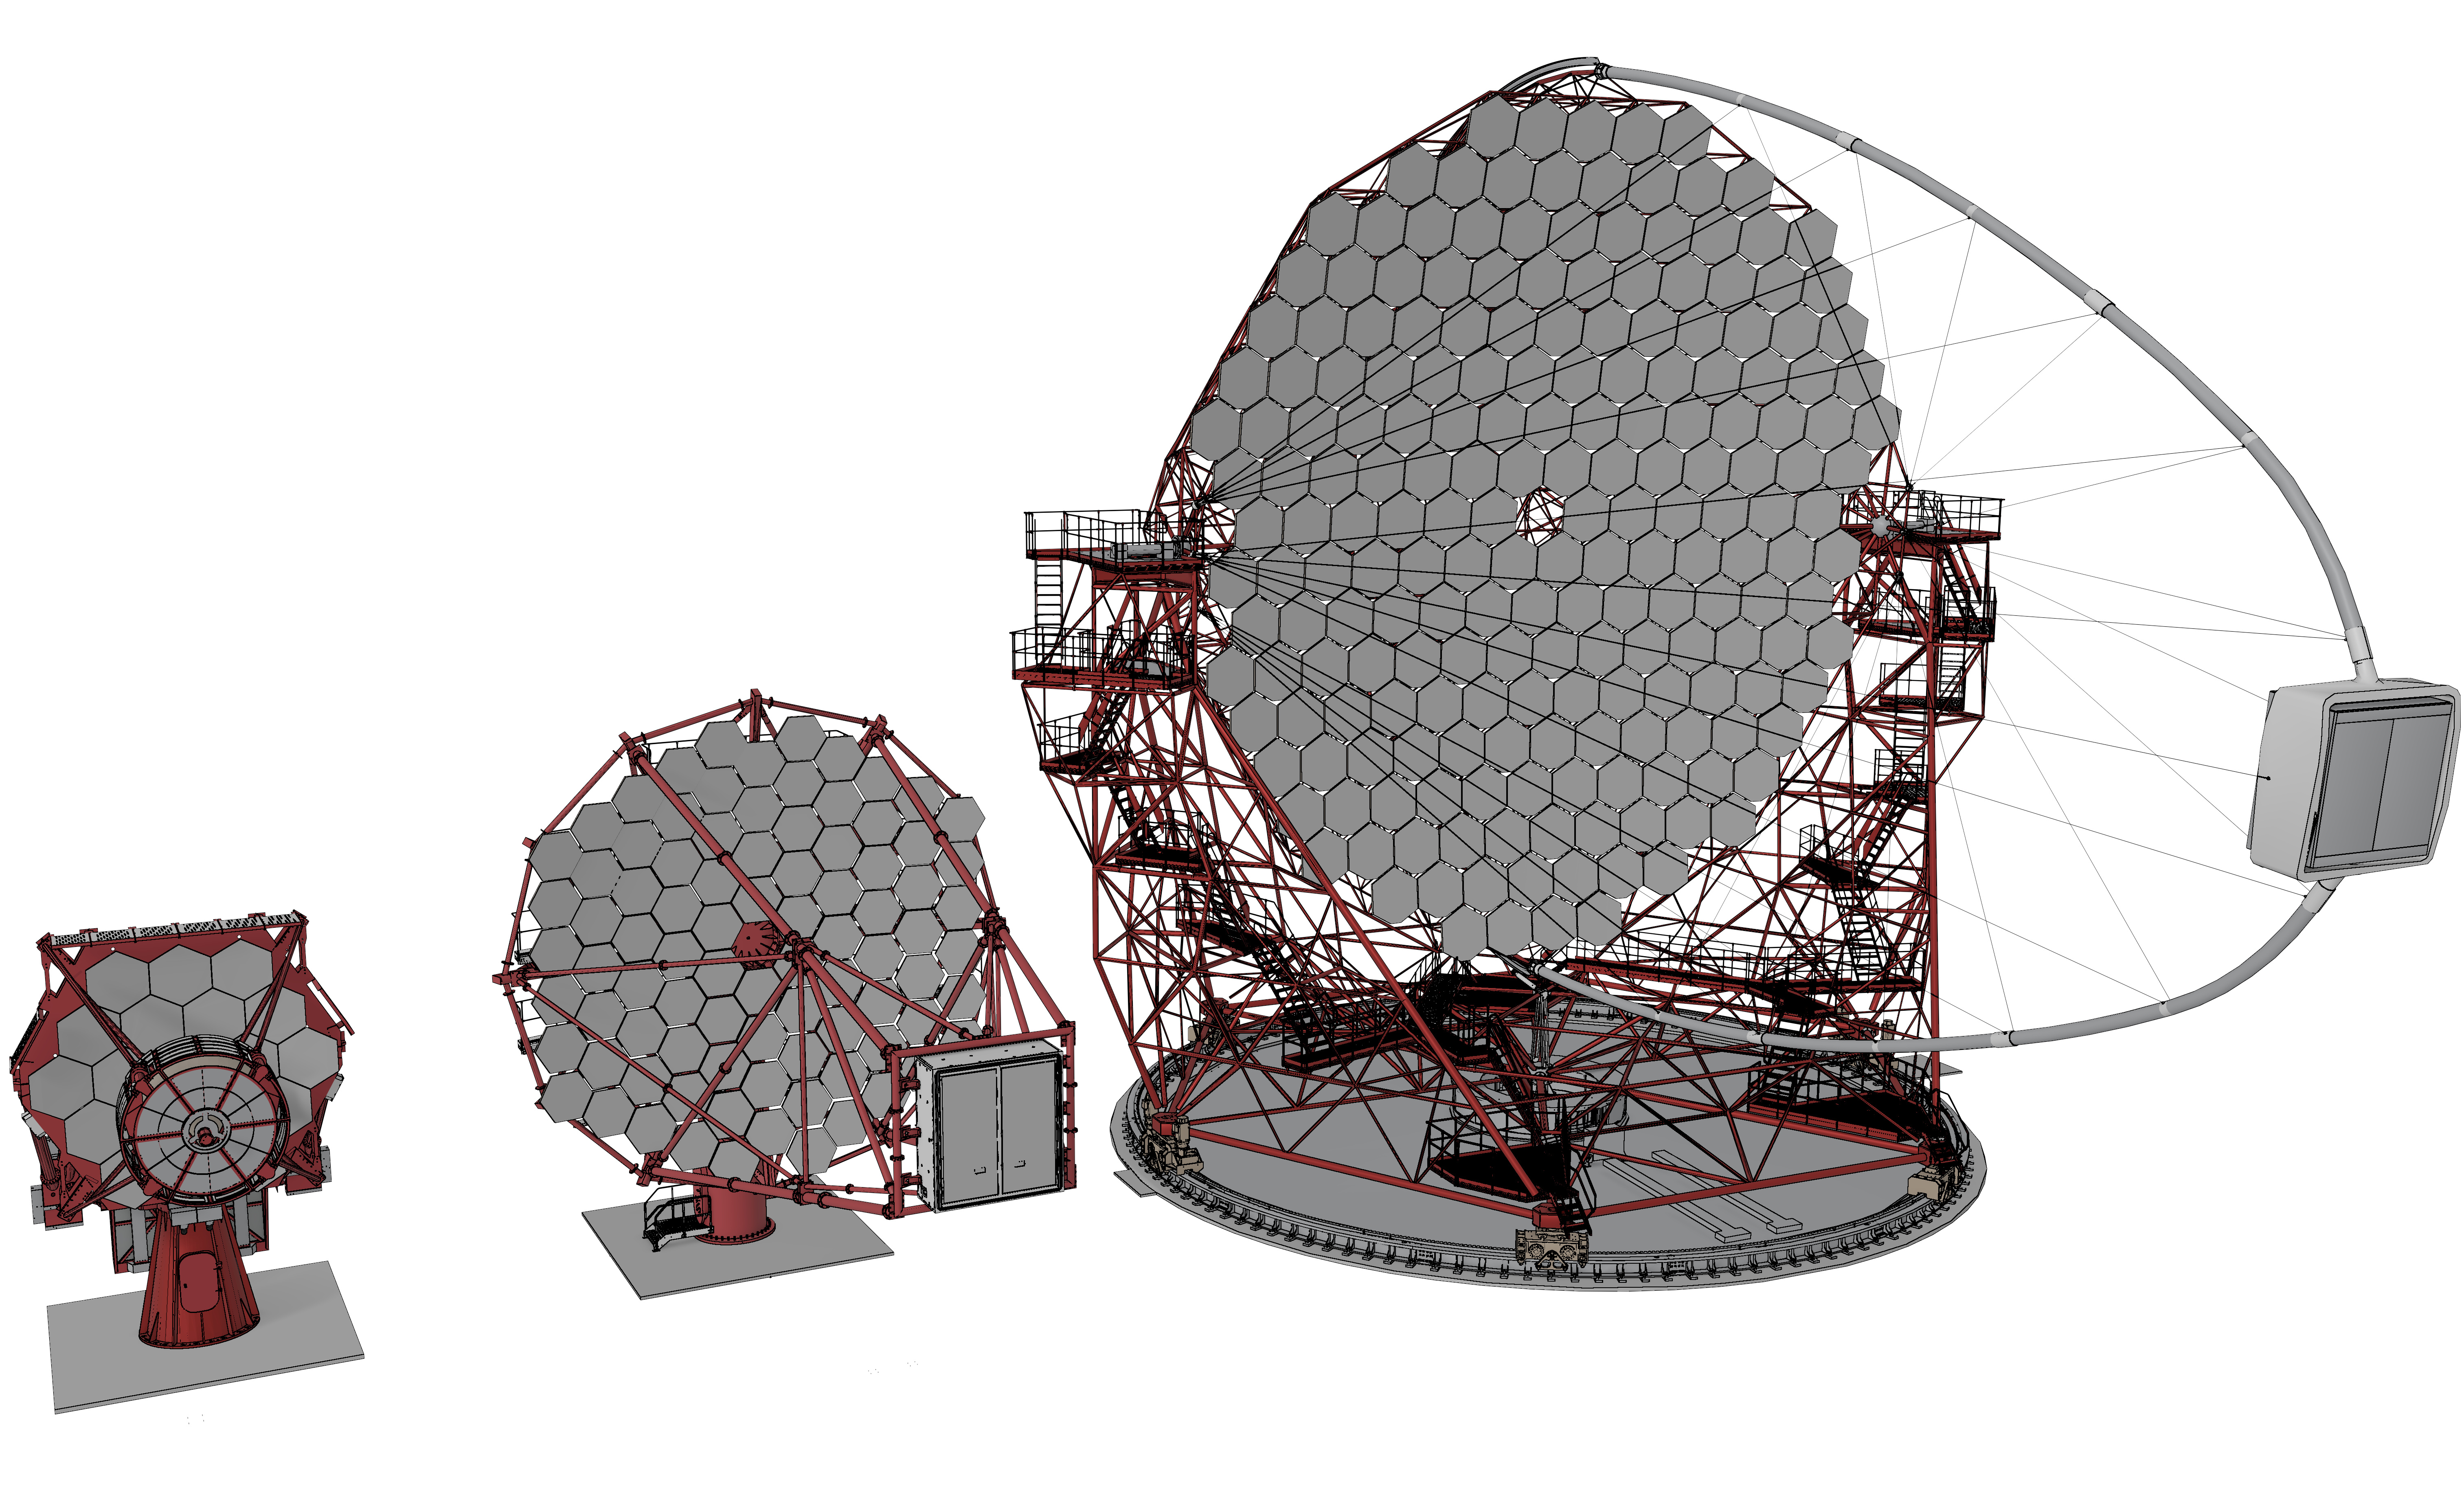
\includegraphics[width=\textwidth]{figures/composite.jpg}
  \caption[Renderings of the individual CTA telescopes]{Renderings of an LST, SST, and MST telescope.
  The LST on the right side has about four times the mirror area of the MST on the left. 
  A prototype of the MST structure was built in Berlin Adlershof where it currently undergoes mechanical testing. 
  Of the three SST prototypes, the ASTRI model will most likely be the one deployed for CTA. 
  The ASTRI telescope is a two-mirror design that allows for a very wide field of view without introducing strong aberration effects.
  All telescopes use active-mirror-control technology that continuously adjusts each individual mirror facet. This helps to compensate 
  for the deformation of the telescope's structure while sources in the sky are being tracked. 
  The LST structure is mounted on bogies running on a flat track of rail with a diameter of approximately \SI{24}{\metre}.
  It weighs a total of 103 tons, of which the camera alone makes up just under 2 tons~\cite{lst_design}. 
  Its slender-looking design is made possible by the use of carbon fiber composite materials.
  This image was rendered using Blender 2.8~\cite{blender} with models provided by G. Pérez Diaz of the Instituto de Astrofísica de Canarias.}
  \label{fig:tel_renders}
\end{figure}

